%% LyX 2.2.3 created this file.  For more info, see http://www.lyx.org/.
%% Do not edit unless you really know what you are doing.
\documentclass[aps,prd,superscriptaddress,nofootinbib,showpacs,showkeys,floatfix]{revtex4}
\usepackage[latin9]{inputenc}
\setcounter{secnumdepth}{3}
\usepackage{color}
\usepackage{amsmath}
\usepackage{amssymb}
\usepackage{graphicx}
\usepackage[unicode=true,
 bookmarks=false,
 breaklinks=false,pdfborder={0 0 1},backref=section,colorlinks=false]
 {hyperref}

\makeatletter

%%%%%%%%%%%%%%%%%%%%%%%%%%%%%% LyX specific LaTeX commands.
%% Because html converters don't know tabularnewline
\providecommand{\tabularnewline}{\\}

%%%%%%%%%%%%%%%%%%%%%%%%%%%%%% Textclass specific LaTeX commands.
\@ifundefined{textcolor}{}
{%
 \definecolor{BLACK}{gray}{0}
 \definecolor{WHITE}{gray}{1}
 \definecolor{RED}{rgb}{1,0,0}
 \definecolor{GREEN}{rgb}{0,1,0}
 \definecolor{BLUE}{rgb}{0,0,1}
 \definecolor{CYAN}{cmyk}{1,0,0,0}
 \definecolor{MAGENTA}{cmyk}{0,1,0,0}
 \definecolor{YELLOW}{cmyk}{0,0,1,0}
}

%%%%%%%%%%%%%%%%%%%%%%%%%%%%%% User specified LaTeX commands.
\PassOptionsToPackage{english}{babel}

\usepackage{float}
\usepackage{mathrsfs}
\usepackage{amsfonts}
\usepackage{array}
\usepackage{epsfig}
% need for subequations
% defines \lesssim, etc
% need for figures
% useful for program listings
% use if color is used in text
%\linespread{1.5}

\renewcommand{\thefootnote}{\fnsymbol{footnote}}
\def\ltap{\raisebox{-.6ex}{\rlap{$\,\sim\,$}} \raisebox{.4ex}{$\,<\,$}}
\def\gtap{\raisebox{-.6ex}{\rlap{$\,\sim\,$}} \raisebox{.4ex}{$\,>\,$}}
\def\lra{\leftrightarrow}
\def\naive{na\"{\i}ve}
\newcommand{\as}{\alpha_{\mathrm{S}}}
\newcommand{\f}[2]{\frac{#1}{#2}}
\def\beq{\begin{equation}}
\def\b0{\beta_0}
\def\bone{\beta_1}
\def\btwo{\beta_2}
\def\eeq{\end{equation}}
\def\beeq{\begin{eqnarray}}
\def\eeeq{\end{eqnarray}}
\def\bom#1{{\mbox{\boldmath $#1$}}}
\def\to{\rightarrow}
\def\ito{\leftarrow}
\def\nn{\nonumber}
\def\arrowlimit#1{\mathrel{\mathop{\longrightarrow}\limits_{#1}}}
\def\qt{q_T}
\newcommand{\asFPi}{\frac{\as}{4\pi}}
\def\ptmin{p_{T{\rm min}}}
\def\ptmax{p_{T{\rm max}}}
\def\ms{${\overline {\rm MS}}$}
\def\tL{{\widetilde L}}
\newcommand{\ib}{\bar{\imath}}

\makeatother

\begin{document}

\preprint{SMU-HEP-?-?}

\title{PDFsense Results}

\author{Bo Ting Wang}

\affiliation{Department of Physics, Southern Methodist University,\\
 Dallas, TX 75275-0181, U.S.A. }

\author{Pavel~M. Nadolsky}

\affiliation{Department of Physics, Southern Methodist University,\\
 Dallas, TX 75275-0181, U.S.A. }
\begin{abstract}
{[}{*} UPDATE THE ABSTRACT {*}{]} % We demonstrate a collection of tools and metrics for quantitatively
% studying the sensitivity of hadronic measurements to the underlying
% Parton Distribution Functions (PDFs). \\
 \\
 \textcolor{red}{Replace PACS with PhySH:}\texttt{\textcolor{red}{https://www.aps.org/publications/apsnews/201602/classification.cfm}} 
\end{abstract}

\pacs{\textcolor{red}{12.15.Ji, 12.38 Cy, 13.85.Qk}}

\keywords{parton distribution functions; Large Hadron Collider; Higgs boson}

\maketitle
\newpage{}\tableofcontents{}\newpage{} % - - - - - - SECTION I - - - - - - - - - - - - - - - - - - - - - - -

\section{Introduction \label{sec:Introduction}}

......

\section{PDF preliminaries \label{sec:PDF-preliminaries}}

\subsection{Data residuals in a global QCD analysis \label{sec:Data-residuals}}

While various theoretical methods exist to compute nucleon PDFs in
terms of models, their unambiguous evaluation in terms of QCD is not
yet possible due to the fact that the PDFs can in general receive
substantial nonperturbative contributions at infrared momenta. For
this reason, precise PDF determination has proceeded mainly through
the technique of the QCD global analysis \textemdash{} a method enabled
by QCD factorization and PDF universality.

In this approach, a highly flexible parametric form is ascribed for
the various flavors in a given analysis at a relatively low scale
$Q_{0}^{2}$. For example, one might take the input PDF for a given
quark flavor $f$ to be an $n$-parameter form 
\begin{equation}
f(x,\mu^{2}=Q_{0}^{2})=A_{f,0}\,x^{A_{f,1}}(1-x)^{A_{f,2}}\,F(x;\,A_{f,3},\dots)\ ,\label{eq:fitform}
\end{equation}
in which $F(x;\:A_{f,3},\dots)$ can be a suitable polynomial function,
\textit{e.g.}, a Chebyshev or Bernstein polynomial, or replaced with
a feed-forward neural network $\mathrm{NN}_{f}(x)$ as in the NNPDF
approach. While the full statistical theory for PDF determination
and error quantification is beyond the intended range of this analysis,
roughly speaking, a best fit is found for a vector $\vec{A}$ of $N$
PDF parameters $A_{l}$ by minimizing a goodness-of-fit function $\chi^{2}$
describing agreement of the QCD data and physical observables computed
in terms of the PDFs. Based on the behavior of $\chi^{2}$ in the
neighbourhood of the global minimum, it is then possible to construct
an ensemble of error PDFs to quantify uncertainties of PDFs at a predetermined
confidence level. 

There are in principle various ways to evaluate uncertainties on PDFs,
\emph{e.g.}, the Hessian method \cite{Pumplin:2001ct,Pumplin:2002vw},
the Monte Carlo method \cite{Giele:1998gw,Giele:2001mr}, and the
Lagrange Multiplier approach \cite{Stump:2001gu}. In this analysis
our default PDF input set is CT14HERA2, which uses the Hessian method
to estimate uncertainties and is therefore based on the quadratic
assumption for $\chi^{2}(\vec{a}$) in the vicinity of the global
minimum at $\vec{a}_{0}$. In the Hessian method, an orthonormal basis
of PDF parameters $\vec{a}$ is derived from the input PDF parameters$\vec{A}$
by the diagonalization of a Hessian matrix $H$, which encodes the
second-order derivatives of $\chi^{2}$ with respect to the physical
PDF model parameters $A_{l}$. The eigenvector PDF combinations $\vec{a}_{l}^{\pm}$are
found for two extreme variations along the direction of the $l$-th
eigenvector of $H$ allowed at a given probability level. The uncertainty
on a QCD observable $X$ can then be estimated with one of available
``master formulas'' \cite[ref to ABM formula with 1 eigenset per direction]{Pumplin:2002vw,Nadolsky:2001yg},
the simplest ``symmetric'' variety of which is 
\begin{align}
\Delta X & =\frac{1}{2}\sqrt{\sum_{l=1}^{N}(X_{l}^{+}-X_{l}^{-})^{2}}\ .\label{DelX}
\end{align}

In the CTEQ-TEA global analysis, the $\chi^{2}$ function accounts
for multiple sources of experimental uncertainties, as well as for
some prior theoretical constraints on the $a_{l}$ parameters. Consequently,
the global $\chi^{2}$ function takes the form 
\begin{equation}
\text{\ensuremath{\chi}}_{global}^{2}=\sum_{E}\chi_{E}^{2}+\chi_{th}^{2},\label{chi2global}
\end{equation}
where the sum runs over all experimental data sets $(E);$ and $\chi_{th}^{2}$
imposes theoretical constraints. The complete formulas for $\chi_{E}^{2}$
and $\chi_{th}^{2}$ can be found in Ref.~\cite{Gao:2013xoa}. For
the purposes of this paper, we express $\chi_{E}^{2}$ for each experiment
$E$ in a compact form as a sum of squared\emph{ shifted residuals}
$r_{i}^{2}(\vec{a})$, which are summed over $N_{pts}$ individual
data points $i$ in this experiment: 
\begin{align}
\chi_{E}^{2}(\vec{a}) & =\sum_{i=1}^{N_{pts}}\,r_{i}^{2}(\vec{a}).\label{eq:chi2}
\end{align}
In turn, $r_{i}(\vec{a})$ for the $i^{th}$ data point is constructed
from the theoretical prediction $T_{i}(\vec{a})$ evaluated in terms
of PDFs, total uncorrelated uncertainty $s_{i}$, and the shifted
central data value $D_{i,sh}(\vec{a})$:
\begin{align}
r_{i}(\vec{a}) & =\frac{1}{s_{i}}\,\big(T_{i}(\vec{a})-D_{i,sh}(\vec{a})\big)\ .\label{eq:residual}
\end{align}

This representation arises because, due to the presence of correlated
systematic errors in many experimental data sets, $\chi_{E}^{2}$
is dependent on $N_{\lambda}$ nuisance parameters $\lambda_{\alpha}$
associated with the correlated systematic factors, in addition to
the PDF parameters $\vec{a}$ and theoretical parameters such as $\alpha_{s}(M_{Z})$
and particle masses. The $\lambda_{\alpha}$ parameters are optimized
for each $\vec{a}$ according to the analytic solution derived in
Appendix B of Ref.~\cite{Pumplin:2002vw}. Optimization effectively
shifts the central value $D_{i}$ of the data point by an amount determined
by the optimal nuisance parameters $\overline{\lambda}_{\alpha}(\vec{a})$
and the correlated systematic errors $\beta_{i\alpha}:$
\begin{equation}
D_{i}\rightarrow D_{i,sh}(\vec{a})=D_{i}-\sum_{\alpha=1}^{N_{\lambda}}\beta_{i\alpha}\overline{\lambda}_{\alpha}(\vec{a}).
\end{equation}
 

We point out that some alternative representations for $\chi^{2}$
include the correlated systematic errors via a covariance matrix $\left(\mbox{cov}\right)_{ij}$,
rather than the above mentioned CTEQ-preferred form that explicitly
operates with $\lambda_{\alpha}$. Various $\chi^{2}$ definitions
in use are reviewed in \cite{Ball:2012wy}, as well as in \cite{Alekhin:2014irh}.
On the other hand, the representations based operating with $\lambda_{\alpha}$
and $\left(\mbox{cov}\right)_{ij}$ are derivable from each other
\cite{Gao:2013xoa}. From an extension of the derivation in Ref.~\cite{Pumplin:2002vw},
we may relate the shifted residual to the covariance matrix at each
individual point as 
\begin{equation}
r_{i}(\vec{a})\ =\ s_{i}\sum_{j=1}^{N_{\mathit{pts}}}(\mathrm{cov}^{-1})_{ij}\,\left(T_{j}(\vec{a})-D_{j}\right),\label{eq:res-cov}
\end{equation}
where 
\begin{equation}
(\mathrm{cov}^{-1})_{ij}\ =\ \left[\frac{\delta_{ij}}{s_{i}^{2}}\,-\,\sum_{\alpha,\beta=1}^{N_{\lambda}}\frac{\beta_{i\alpha}}{s_{i}^{2}}A_{\alpha\beta}^{-1}\frac{\beta_{j\beta}}{s_{j}^{2}}\right]\ ,\label{eq:covmat}
\end{equation}
and 
\begin{equation}
A_{\alpha\beta}\ =\ \delta_{\alpha\beta}\,+\,\sum_{k=1}^{N_{\mathit{pts}}}\frac{\beta_{k\alpha}\beta_{k\beta}}{s_{k}^{2}}\ .
\end{equation}
Thus, even if the PDF analyses operates with the covariance matrix,
one is still able to determine the shifted residuals $r_{i}$ from
$\left(\mbox{cov}^{-1}\right)_{ij}$ using Eq.~(\ref{eq:res-cov}).
In this article, we conveniently follow the CTEQ methodology and obtain
$r_{i}(\vec{a})$ directly from the CTEQ-TEA fitting program, together
with optimal nuisance parameters $\overline{\lambda}_{\alpha}(\vec{a})$
and shifted central data values $D_{i,sh}(\vec{a}).$

\subsection{Visualization of the global fit with the help of residuals}

......

\clearpage\newpage

\section{Quantifying distributions of residuals\label{sec:QuantifyingDistributionsOfResiduals}}

We have demonstrated that the multi-dimensional distribution of the
shifted residuals $r_{i}$ evaluated with Hessian eigenvector PDFs
reflects PDF dependence of individual data points. In this section,
we will focus on numerical metrics to assess the emerging geometrical
picture and to visualize the regions of partonic momentum fractions
$x$ and QCD factorization scales $\mu$ where the experiments impose
strong constraints on a given PDF-dependent observable $X$. 

\subsection{Reciprocated distances \label{sec:Reciprocated-distances}}

\subsection{Correlations and sensitivities \label{sec:CorrelationsSensitivities}}

Next, we examine gradients of $r_{i}$ in space of eigenvector PDF
parameters $\vec{a},$ where they are naturally related to to the
PDF uncertainty in the Hessian approach. Recall that in the Hessian
method the PDF uncertainty on $X(\vec{a})$ is found as 
\begin{equation}
\Delta X(\vec{a})=X(\vec{a})-X(\vec{a}_{0})=\vec{\nabla}X|_{\vec{a}_{0}}\cdot\Delta\vec{a},
\end{equation}
where $\vec{a}_{0}$ is the best-fit combination of PDF parameters,
and $\Delta\vec{a}$ is the maximal displacement along the gradient
that is allowed within the tolerance hypesphere of radius $T$ centered
on the best fit \cite{Pumplin:2001ct,Pumplin:2002vw}. The standard
master formula 
\begin{equation}
\Delta X=\left\vert \vec{\nabla}X\right\vert =\frac{1}{2}\sqrt{\sum_{l=1}^{N}\left(X_{l}^{+}-X_{i}^{-}\right)^{2}}\label{masterDX-1}
\end{equation}
is obtained by representing the components of $\vec{\nabla}X$ by
a finite-difference formula 
\begin{equation}
\frac{\partial X}{\partial a_{i}}=\frac{1}{2}(X_{i}^{+}-X_{i}^{-}),\label{dXdzi-1-1}
\end{equation}
in terms of the values $X_{l}^{\pm}$ for extreme displacements of
$\vec{a}$ within the tolerance hypersphere along the $l$-th direction. 

In this setup, a dot product between the gradients provides a convenient
measure of the degree of similarity between PDF dependence of two
quantities \cite{Nadolsky:2008zw}. A dot product $\vec{\nabla}r_{i}\cdot\vec{\nabla f}$
between the gradients of a shifted residual $r_{i}$ and another QCD
variable $f$, such as the PDF at some $\{x,\mu\}$ or a cross section,
can be cast in a number of useful forms.

\subsubsection{Correlation cosine. }

The correlation, which we define following Refs.~\cite{Pumplin:2001ct,Nadolsky:2001yg,Nadolsky:2008zw,Gao:2017yyd}
according to 
\begin{equation}
C_{f}\,\equiv\,\mbox{Corr}[f,r_{i}]=\frac{\vec{\nabla f}\cdot\vec{\nabla r}_{i}}{\Delta f\,\Delta r_{i}},\label{eq:corr}
\end{equation}
encodes the quantitative relation between $f$ and $r_{i}$ and can
determine whether there \emph{can} exist a predictive relationship
between $f$ and goodness of fit to the $i$-th data point. The correlation
function $\mathrm{\mbox{Corr}}[X,Y]$ of the quantities $X,\,Y$ in
Eq.~(\ref{eq:corr}) represents the Hessian formalism realization
of the Pearson's correlation coefficient, which we express as 
\begin{align}
\mathrm{\mbox{Corr}}[X,Y] & =\frac{1}{4\Delta X\Delta Y}\sum_{j=1}^{N}(X_{j}^{+}-X_{j}^{-})(Y_{j}^{+}-Y_{j}^{-})\ ,\label{eq:corr-def}
\end{align}
the sum in these expressions being over the $j$ parameters of the
full PDF model space. Geometrically, $\mbox{Corr}[X,Y]$ represents
the cosine of the angle that determines the eccentricity of an ellipse
satisfying $\chi^{2}(\vec{a})<\chi^{2}(\vec{a}_{0})+T^{2}$ in the
$\{X,Y\}$ plane. This latter point follows from the fact that the
mapping of the tolerance hypersphere onto the $\{X,Y\}$ plane is
an ellipse, its eccentricity depends on the correlation of $X$ and
$Y,$ which in turn is given by Eq.~(\ref{eq:corr-def}) above. 

$\mbox{Corr}[r_{i},f]$ does not indicate how constraining the residual
is, but it may indicate a predictive relation between $r_{i}$ and
$f$ with a large enough magnitude of the (anti-)correlation. From
the past experience, we could say that the (anti-)correlation between
$X$ and $Y$ is significant roughly if $\left|\mbox{Corr}[X,Y]\right|\gtrsim0.7.$
Smaller (anti-)correlation values are less robust or predictive. Following
this rule-of-thumb, correlations have been used successfully to identify
PDF combinations that dominate PDF uncertainties of complicated observables,
for instance to show that the gluon uncertainty dominates the total
uncertainty on LHC $W$ and $Z$ production, or that the uncertainty
on the ratio $\sigma_{W}^{\pm}/\sigma_{Z}$ of $W$ and $Z$ cross
sections at the LHC is dominated by the strangeness PDF, rather than
$u$ and $d$ (anti-)quark PDFs \cite{Nadolsky:2008zw}. 

\subsubsection{Sensitivity.}

While the correlation $C_{f}$ can provide insight into the relationship
between the PDF dependences of a prediction for the $i$-th data point
and a QCD function $f$, it alone does not fully quantify the extent
to which an individual data point constrains the fit uncertainty.
Similarly, it does not encode by itself the potential impact of separate
or new measurements on improving PDF determinations in terms of the
uncertainty reduction. For this purpose, we employ $\vec{\nabla f}\cdot\vec{\nabla r}_{i}$
again to define the \textit{sensitivity} of the $i^{th}$ data point
to $f$, 
\begin{equation}
S_{f}\equiv\frac{\vec{\nabla f}\cdot\vec{\nabla r}_{i}}{\Delta f\,\langle r_{0}\rangle_{E}}=\frac{\Delta r_{i}}{\langle r_{0}\rangle_{E}}\,C_{f}\ ,\label{eq:sens}
\end{equation}
where $\Delta r_{i}$ and $\langle r_{0}\rangle_{E}$ are computed
according to Eqs.~(\ref{DelX}) and (\ref{r0E}), respectively. In
other words, $\Delta r_{i}$ represents the variation of the residuals
across the set of Hessian error PDFs, which we normalize to the root-mean-squared
residual for a given experiment to reduce impact of random fluctuations
of the experimental data values $D_{i}$. This definition has the
benefit of encoding not only the correlated relationship of $f$ with
the residual, but also the comparative size of the experimental uncertainty
with respect to state-of-the-art PDF uncertainties. In consequence,
for example, if a new experimental data have reported uncertainties
that are much tighter than the present PDF errors, these data would
register as high-sensitivity points by the definition in Eq.~(\ref{eq:sens}). 

Geometrically, $S_{f}$ represents a projection of the displaced residual
vector $\vec{\delta_{i}}$, defined in Sec.~\ref{sec:QuantifyingDistributionsOfResiduals}
using the symmetrized formula for $\delta_{il}$ from footnote \ref{fn:sym-deltail},
onto the direction of the gradient $\vec{\nabla}f$. This interpretation
suggests that the strength of constraints from the global data set
along the direction of $\vec{\nabla}f$ can be quantified by summing
projections $S_{f}$ for individual $\vec{\delta}_{i}$ of all contributing
data points onto the direction of$\vec{\nabla}f$. 

As with correlations, only a sufficiently large absolute magnitude
of $\left|S_{f}\right|$ is indicative of a predictive constraint
of the $i$-th point on $f$. Recall that $r_{i}^{2}$ is the contribution
of the $i$-th point to $\chi^{2},$ and that only residuals with
a large enough $\Delta r_{i}$, as compared to the r.m.s. residual
$\langle r_{0}\rangle_{E}$, are sensitive to PDF variations. The
$S_{f}$ magnitude is of order $\Delta r_{i}/\langle r_{0}\rangle_{E},$
which suggests an estimate of a minimal value of $S_{f}$ that would
be deemed sensitive according to the respective $\chi^{2}$ contribution.
For the numerical comparisons in this study, we assume that $\left|S_{f}\right|$
must be no less than 0.25 to indicate a predictive constraint, as
the PDF uncertainty of the $i$-th residual contributes no less than
0.0625 to the variation in the global $\chi^{2}$. The minimal value
can be adjusted depending on accuracy. 

Yet another possible definition, which we list for completeness, is
to normalize the sensitivity as 
\begin{equation}
S_{f}^{\prime}\equiv\frac{\vec{\nabla f}\cdot\vec{\nabla r}_{i}}{f_{0}\,\langle r_{0}\rangle_{E}}=\frac{\Delta f}{f_{0}}\,S_{f}\ .\label{eq:sens-prime}
\end{equation}
For instance, if $f$ is the PDF $f(x_{i},\mu_{i})$ at the same points
$\{x_{i},\mu_{i}\}$ as the data, the definition (\ref{eq:sens-prime})
de-emphasizes $S_{f}^{\prime}$ at those data points where the PDF
uncertainty$\Delta f(x_{i},\mu_{i})$ is small compared to the best-fit
PDF value $f_{0}(x_{i},\mu_{i})$. 

\clearpage\newpage

\section{Case study: CTEQ-TEA global data \label{sec:CaseCTEQ-TEA}}

\subsection{Maps of correlations and sensitivities}

......

\subsection{Experiment rankings according to cumulative sensitivities \label{sec:Experiment-rankings-according}}

......

\section{Case study: various Processes in CTEQ-TEA Data}

\subsection{All processes in CT14 HERA2 + LHC new data}

...
\begin{enumerate}
\item showing all experiments at (x,Q) space of PDFs \ref{fig:all_expt_xQ_data}
\item shows correlation, sensitivity, and respective histograms \ref{fig:CorrSensH14},
\ref{fig:Corrgluon}, \ref{fig:Sensgluon}
\item sensitivity to Higgs cross section at 14 TeV indicate the PDF sensitive
to the future LHC Higgs survey \ref{fig:CorrSensH14} 
\item sensitivity to gluon PDF shows demonstrate that constraint of gluon
at small x region (10\textasciicircum{}-3\textasciitilde{}-5) is from
HERA2 data and LHC jet data provides fluent constaint to gluon at
x\textgreater{}10\textasciicircum{}-3 \ref{fig:Corrgluon}, \ref{fig:Sensgluon}
\end{enumerate}
\begin{figure*}
\includegraphics[width=1\textwidth]{plots/processes/all_expt/Allexpt_xQbyexpt_xQ}
\caption{A graphical representation in $\{x,\mu\}$ space of the full data
set treated in the present analysis, designated as ``CTEQ-TEA''.
It corresponds to an expansion of the CT14HERA2 data \cite{Hou:2016nqm}
fitted in the most recent CT14 framework \cite{Dulat:2015mca}, including
measurements from Run II of HERA \cite{Abramowicz:2015mha}. }
\label{fig:all_expt_xQ_data} 
\end{figure*}

\begin{figure*}
\includegraphics[width=0.49\textwidth]{plots/processes/all_expt/Allexpt_corr_xQ+1_f8_samept}\ \ \
\includegraphics[width=0.48\textwidth]{plots/processes/all_expt/Allexpt_corrdr_xQ+1_f8_samept}
\caption{For the full CTEQ-TEA dataset of Fig.~\ref{fig:all_expt_xQ_data},
we show the absolute correlation $|C_{f}|$ and sensitivity $|S_{f}|$
associated with the 14 TeV Higgs production cross section $\sigma_{H^{0}}(14\,\mathrm{TeV})$.
Points with significant magnitudes of $|C_{f}|$ and $|S_{f}|$ are
highlighted with color. When only the $|C_{f}|$ plot at left is considered,
it is primarily a subpopulation of jet production data (diagonal open
and closed inverted triangles with $\mu\gtrsim100$ GeV) that exhibits
significant correlations, as well as some HERA DIS and $t\bar{t}$
production data points. Our novel definition for the sensitivity in
the right panel, on the other hand, reveals many more points that
have comparable potency for constraining the Higgs cross section.
In this case, the great bulk of the jet production points, including
many of the highest scale measurements, is important, as well as a
number of other processes at smaller $\mu$, such as DIS data from
HERA (Exp. ID 160), NMC (104) and CDHSW (108), Drell-Yan information
from E866 (204), $t\bar{t}$ (565-568) and high-$p_{T}$ $Z$ production,
and even some points obtained from $Z$ production at LHCb (246).
\label{fig:CorrSensH14}}
\end{figure*}

\begin{figure*}
\includegraphics[width=0.49\textwidth]{plots/processes/all_expt/corr_xQ+1_f0_samept_nohigh}\ \ \
\includegraphics[width=0.48\textwidth]{plots/processes/all_expt/Allexpt_corr_hist+1_f0_samept}
\caption{Two representations of the correlation $|C_{g}|(x_{i},\mu_{i})$ of
the gluon PDF $g(x,\mu)$ with the point-wise residual $r_{i}$ of
the augmented CT14HERA2 analysis; in the left panel we plot a histogram
showing the distribution of correlations over 5227 $\{x,\mu\}$ points.
In the right panel we show the $\{x_{i},\mu_{i}\}$ map of these correlations
for the full dataset. \label{fig:Corrgluon}}
\end{figure*}

\begin{figure*}
\includegraphics[width=0.49\textwidth]{plots/processes/all_expt/corrdr_xQ+1_f0_samept_nohigh}\ \ \
\includegraphics[width=0.48\textwidth]{plots/processes/all_expt/Allexpt_corrdr_hist+1_f0_samept}
\caption{Like Fig.\ref{fig:Corrgluon}, but for the gluon sensitivity $|S_{g}|(x_{i},\mu_{i})$
as defined in Eq.\textasciitilde{}(\textbackslash{}ref\{eq:sens\}).
\label{fig:Sensgluon}}
\end{figure*}

\subsection{DIS NC processes}

\subsection{DIS CC processes}

\subsection{HERA Run 2 (ID = 160)}

\subsection{Jet, $t\overline{t}$ and Zpt Processes}

......
\begin{enumerate}
\item jet CMS and ATLAS data provide the most fluent sensitivity to gluon,
b, c, and Higgs processes \ref{fig:jet_ttbar_Zpt_new}
\item Although ttbar and Zpt are also averagely sensitive to these flavours,
they are not necessary when we incorporate LHC jet data sets \ref{fig:jet_ttbar_Zpt_new}. 
\end{enumerate}
\begin{figure*}
\includegraphics[clip,width=0.45\textwidth]{plots/processes/jet/new/corrdr_xQ+1_f0_samept}
\ \ \
\includegraphics[clip,width=0.45\textwidth]{plots/processes/jet/new/corrdr_xQ+1_f8_samept} 

\includegraphics[clip,width=0.45\textwidth]{plots/processes/ttbar/corrdr_xQ+1_f8_samept}
\ \ \
\includegraphics[clip,width=0.45\textwidth]{plots/processes/Zpt/corrdr_xQ+1_f8_samept} 

\caption{left-up and right-up are jet (542, 544, 545). left-down is ttbar (565\textasciitilde{}568).
right-down is Zpt (247, 253, 254, 255) events.}
\label{fig:jet_ttbar_Zpt_new}
\end{figure*}

\subsection{$W$ processes}
\begin{enumerate}
\item new data (249) impose d, dbar, d/u, dbar/ubar constraints \ref{fig:W_new}
\end{enumerate}
\begin{figure*}
\includegraphics[clip,width=0.45\textwidth]{plots/processes/W/new/corrdr_xQ+1_f2_samept}
\ \ \
\includegraphics[clip,width=0.45\textwidth]{plots/processes/W/new/corrdr_xQ+1_f13_samept} 

\caption{LHC W asymmetry data (249) }
\label{fig:W_new}
\end{figure*}

\subsection{$Z$ processes}

\section{Case Study: LHeC \label{sec:Case-Study:-LHeC}}

......Here provide the prediction of the sensitivity analysis of LHeC
DIS NC and CC data sets \ref{tab:LHeC} 
\begin{enumerate}
\item LHeC DISNC data constrains small x gluon \ref{fig:LHeC-sens}, \ref{fig:LHeC-corr}
\item LHeC DISCC and DISNC data constrain u and d large x and small x. For
the small x region, the high sensitivity results from the few constraint
before LHC data
\item LHeC DISCC data is correlated to middle x region (10\textasciicircum{}-3\textasciitilde{}10\textasciicircum{}-2)
s PDF, I don't know why \ref{fig:LHeC-corr}
\item don't know why the 192 (CC), 194 (NC) are strongly correlated with
the diagonal part of ubar PDF \ref{fig:LHeC-corr}
\item large $\delta r$ enhance the sensitivities of LHeC data to PDFs especially
at small x region \ref{fig:LHeC-dr}
\end{enumerate}
\begin{figure*}
\includegraphics[clip,width=0.45\textwidth]{plots/LHeC/corrdr_xQ+1_f0_samept}
\ \ \
\includegraphics[clip,width=0.45\textwidth]{plots/LHeC/corrdr_xQ+1_f2_samept} 

\includegraphics[clip,width=0.45\textwidth]{plots/LHeC/corrdr_xQ+1_f3_samept}
\ \ \
\includegraphics[clip,width=0.45\textwidth]{plots/LHeC/corrdr_xQ+1_f-1_samept} 

\caption{Select sensitivity plots for the LHeC pseudodata, in this case showing
$|S_{g}|(x_{i},\mu_{i})$ in the left-up panel, $|S_{d}|(x_{i},\mu_{i})$
in the right-up, $|S_{s}|(x_{i},\mu_{i})$ in the left-down, and $|S_{\overline{u}}|(x_{i},\mu_{i})$
in the right-down. The pseudodata are broken among four separate reaction
channels \textemdash{} CC $e^{-}p$ (circles) and $e^{+}p$ (squares),
as well as NC $e^{-}p$ (diamonds) and $e^{+}p$ (triangles). }
\label{fig:LHeC-sens} 
\end{figure*}

\begin{figure*}
\includegraphics[clip,width=0.45\textwidth]{plots/LHeC/corr_xQ+1_f0_samept}
\ \ \
\includegraphics[clip,width=0.45\textwidth]{plots/LHeC/corr_xQ+1_f2_samept} 

\includegraphics[clip,width=0.45\textwidth]{plots/LHeC/corr_xQ+1_f3_samept}
\ \ \
\includegraphics[clip,width=0.45\textwidth]{plots/LHeC/corr_xQ+1_f-1_samept} 

\caption{Select correlation plots for the LHeC pseudodata, in this case showing
$|C_{g}|(x_{i},\mu_{i})$ in the left-up panel, $|C_{d}|(x_{i},\mu_{i})$
in the right-up, $|C_{s}|(x_{i},\mu_{i})$ in the left-down, and $|C_{\overline{u}}|(x_{i},\mu_{i})$
in the right-down. The pseudodata are broken among four separate reaction
channels \textemdash{} CC $e^{-}p$ (circles) and $e^{+}p$ (squares),
as well as NC $e^{-}p$ (diamonds) and $e^{+}p$ (triangles). }
\label{fig:LHeC-corr} 
\end{figure*}

\begin{figure*}
\includegraphics[clip,width=0.45\textwidth]{plots/LHeC/dr_xQ+1_samept}
\ \ \
\includegraphics[clip,width=0.45\textwidth]{plots/LHeC/dr_hist+1_samept} 

\caption{Select $\delta r$ plots for the LHeC pseudodata, in this case showing
$\delta r_{i}$ in the left panel and $\delta r_{i}$ histogram in
the right. The pseudodata are broken among four separate reaction
channels \textemdash{} CC $e^{-}p$ (circles) and $e^{+}p$ (squares),
as well as NC $e^{-}p$ (diamonds) and $e^{+}p$ (triangles). }
\label{fig:LHeC-dr} 
\end{figure*}

......

\begin{table}[ht]
\begin{tabular}{|l|lr|c|c}
\hline 
\textbf{ID\#}  & \textbf{LHeC pseudodata set}  &  & $N_{pts}$  & Fig.~\ref{fig:LHeC} symbol \tabularnewline
\hline 
\hline 
191  & CC $e^{-}p$  &  & 93  & circle \tabularnewline
\hline 
192  & CC $e^{+}p$  &  & 109  & square \tabularnewline
\hline 
193  & NC $e^{-}p$  &  & 128  & diamond \tabularnewline
\hline 
194  & NC $e^{+}p$  &  & 148  & triangle \tabularnewline
\hline 
\end{tabular}\caption{Separate channels of the unpolarized lepton-proton deep-inleastic
scattering pseudodata for the LHeC from Ref.~\cite{LHeCdata}. For
each channel, here we list the specific physical process, number of
associated pseudodata points, as well as the symbol indicating the
channel in the $|S_{f}|(x_{i},\mu_{i})$ plots of Fig.~\ref{fig:LHeC}. }
\label{tab:LHeC} 
\end{table}

\section{Case Study: Mellin Moment }

......Compare with lattice predictions and constrain parametrization
function by penalty
\begin{enumerate}
\item B-C and gluon are sensitive to jet data \ref{fig:Mellin_B-C}
\item $(u^{-}-d^{-})x^{0}$ should be 1 (constant) but it's total sensitivity
is the same amount compared with other Mellin moments \ref{tab:Mellin_total_sens}.
We can lower the order of precision to reduce the flutuation. However,
it also indicates even an physical quantity has no correlation/sensitivity
with data sets/PDFs, the numerical fluctuation still impose some sensitivity.
Therefore, perhaps we don't want to consider too low sensitivity as
the real sensitivity.
\item some Mellin moments are sensitive to data at a narrow x band \ref{fig:Melling_x-1x0},
\ref{fig:Mellin_x2x3}. This perhaps indicates that Mellin moments
could be well-measured by just constraining PDFs at specific regions. 
\end{enumerate}
\textcolor{red}{note: the total sensitivity table uses the old formula,
it should be modify latter}

\begin{figure*}
\includegraphics[clip,width=0.45\textwidth]{plots/MellinMoment/corrdr_xQ+1_f55_samept}
\ \ \
\includegraphics[clip,width=0.45\textwidth]{plots/MellinMoment/corr_xQ+1_f55_samept} 

\includegraphics[clip,width=0.45\textwidth]{plots/MellinMoment/corrdr_xQ+1_f57_samept}
\ \ \
\includegraphics[clip,width=0.45\textwidth]{plots/MellinMoment/corr_xQ+1_f57_samept} 

\caption{data sets sensitivity to the 1st and 3rd order B-C of Melling moment}
\label{fig:Mellin_B-C} 
\end{figure*}

\begin{table}[ht]
\begin{tabular}{|l|lr}
\hline 
\textbf{ID\#}  & \textbf{\textbar{}S\textbar{}}  & \textbar{}S\textbar{} for the respective quantities\tabularnewline
\hline 
\hline 
most  & 350\textasciitilde{}450 & 500\textasciitilde{}1000\tabularnewline
\hline 
$(u^{-}-d^{-})x^{0}$ & 418. & 590.\tabularnewline
\hline 
B-C\textasciicircum{}2 & 788. & 928.\tabularnewline
\hline 
B-C\textasciicircum{}3 & 848. & 928.\tabularnewline
\hline 
T15\textasciicircum{}2 & 501. & 843.\tabularnewline
\hline 
T15\textasciicircum{}3 & 530. & 843.\tabularnewline
\hline 
T24\textasciicircum{}3 & 536. & 826.\tabularnewline
\hline 
g\textasciicircum{}2 & 794. & 907.\tabularnewline
\hline 
g\textasciicircum{}3 & 851. & 907.\tabularnewline
\hline 
\end{tabular}\caption{high total sensitivity to mellin moments of quantities and the respective
non-mellin moment quantitives}
\label{tab:Mellin_total_sens} 
\end{table}

\begin{figure*}
\includegraphics[clip,width=0.45\textwidth]{plots/MellinMoment/x0x-1_corr/corr_xQ+1_f28_samept}
\ \ \
\includegraphics[clip,width=0.45\textwidth]{plots/MellinMoment/x0x-1_corr/corr_xQ+1_f29_samept} 

\includegraphics[clip,width=0.45\textwidth]{plots/MellinMoment/x0x-1_corr/corr_xQ+1_f48_samept}
\ \ \
\includegraphics[clip,width=0.45\textwidth]{plots/MellinMoment/x0x-1_corr/corr_xQ+1_f49_samept} 

\caption{data sets sensitivity to x\textasciicircum{}-1, x\textasciicircum{}0
of Melling moment }
\label{fig:Melling_x-1x0} 
\end{figure*}

\begin{figure*}
\includegraphics[clip,width=0.45\textwidth]{plots/MellinMoment/x2x3_corr/corr_xQ+1_f18_samept}
\ \ \
\includegraphics[clip,width=0.45\textwidth]{plots/MellinMoment/x2x3_corr/corr_xQ+1_f19_samept} 

\includegraphics[clip,width=0.45\textwidth]{plots/MellinMoment/x2x3_corr/corr_xQ+1_f21_samept}
\ \ \
\includegraphics[clip,width=0.45\textwidth]{plots/MellinMoment/x2x3_corr/corr_xQ+1_f22_samept} 

\caption{data sets sensitivity to x\textasciicircum{}2, x\textasciicircum{}3
of Melling moment}
\label{fig:Mellin_x2x3} 
\end{figure*}

\section{Case Study: comparison of the fit with jets and with no jets}

...HERA2 and HERA2NoJet are fit with jet data sets (504, 514, 535,
538) and without jet data sets. Here we compare the difference of
sensitivities to PDFs for HERA2 and HERA2NoJet.
\begin{enumerate}
\item this comparison shows the possible sensitivity impacts when incorporate
data sets in the fit of PDF sets \ref{tab:HERA2_HERA2NoJet_total_sens},
\ref{fig:HERA2_HERA2NoJet_r_dr}, \ref{fig:HERA2_HERA2NoJet_corr_sens}
\item after fit with jet data, both total correlation and dr reduce, so
the total sensitivity is pulled down.
\item changes are mainly in jet data (the total sensitivity difference are
mostly from jet old and new data), so the old jet data in the fit
actually mostly constrain the PDF space associated with jet processes
\item ttbar and Zpt gluon are also constrained, because the constrained
space associated with jet processes is close to the space of ttbar/Zpt
processes, which is mainly associated with gluon PDF.
\item reciprocate distance formula: $rd_{i}=(Npt-N_{sameID}/Npt)*1/(\sum_{i_{ID}\text{\ensuremath{\neq}}j_{ID}}^{Npt}|\stackrel{\rightharpoonup}{v_{i}}-\stackrel{\rightharpoonup}{v_{j}}|)$,
where $\stackrel{\rightharpoonup}{v_{i}}$ is the vector of PCA-reduced
10 dimensions of the normalized residual ($\stackrel{\rightharpoonup}{\delta r}/r_{ID,rms}$)
in Hessian-replica space. The comparison of reciprocate distances
of normalized residuals of data sets to HERA2 and HERA2NoJet shows
that 234, 266, 203 are in average more far away to other data in the
replica space of normalized residuals \ref{fig:HERA2_HERA2NoJet_rd3}.
The ranking of distances for two PDF sets are similar, indicating
that the fits with jet data sets (504, 514, 535, 538) does not constrain
the similar space of PDFs to other experiments. In the LHC data sets,
245, 249, 250, 542, 545 perhaps discover more new PDF space than others.
For the experiments with most points that are far away from other
points at space
\item apply PCA and t-SNE algorithm to $\stackrel{\rightharpoonup}{\delta r}/r_{ID,rms}$,
we can efficiently separate it to different types, which means these
algorithm illustrates the difference of PDF-space constraint from
data sets \ref{fig:PCA_t-SNE}. 
\end{enumerate}
\textcolor{red}{note: 1. The title of HERA2NoJet figures \ref{fig:HERA2_HERA2NoJet_rd3}
are not correct, which is still ``CT14HERA2 NNLO''. 2. Because I
use the plotted data with multiple points specified by .dta points,
the distances estimation of VBP, Jet, ttbar data are not correct.
I should use the normalized residuals of .dta data to calculate the
reciprocate distance. }

\begin{table}[ht]
\begin{tabular}{|l||llrrrrrrrrrrr}
\hline 
\textbf{ID\#}  & Npt & \textbf{\textbar{}r\textbar{}yes}  & \textbf{\textbar{}r\textbar{}no}  & \textbf{\textbar{}dr\textbar{}yes}  & \textbf{\textbar{}dr\textbar{}no}  & \textbf{\textbar{}Cg\textbar{}yes}  & \textbf{\textbar{}Cg\textbar{}no}  & \textbf{\textbar{}Sg\textbar{}yes}  & \textbf{\textbar{}Sg\textbar{}no}  & \textbf{\textbar{}Cs\textbar{}yes}  & \textbf{\textbar{}Cs\textbar{}no}  & \textbf{\textbar{}Ss\textbar{}yes}  & \textbf{\textbar{}Ss\textbar{}no} \tabularnewline
\hline 
\hline 
All & 5227 & 4857. & 5345. & 3835. & 4979. & 1398. & 1636. & 847. & 1215. & 693. & 901. & 450. & 677.\tabularnewline
\hline 
jet old  & 666 & 478. & 554. & 266. & 537. & 242. & 298. & 106. & 224. & 79. & 140. & 33. & 103.\tabularnewline
\hline 
jet new & 804 & 860. & 1250. & 874. & 1707. & 390. & 420. & 337. & 522. & 135. & 195. & 117. & 230.\tabularnewline
\hline 
ttbar & 35 & 26. & 43. & 18. & 34. & 18. & 20. & 10. & 14. & 3.9 & 3.7 & 2.1 & 2.6\tabularnewline
\hline 
Zpt & 53 & 79. & 82. & 26. & 32. & 25. & 32. & 6.5 & 11.1 & 18. & 16. & 5.6 & 5.7\tabularnewline
\hline 
\end{tabular}\caption{Total sensitivities comparison of HERA2 and HERA2NoJet. jet old: 504,
514, 535, 538. All: HERA2 data + new data (LHC jet, ttbar, Zpt, W/Z).
jet new: 42, 544, 545. ttbar: 565, 566, 567, 568. Zpt: 247, 253, 254,
255 }
\label{tab:HERA2_HERA2NoJet_total_sens} 
\end{table}

\begin{figure*}
\includegraphics[clip,width=0.45\textwidth]{plots/HERA2_HERA2NoJet/HERA2/residual_xQ+1_samept}
\ \ \
\includegraphics[clip,width=0.45\textwidth]{plots/HERA2_HERA2NoJet/HERA2NoJet/residual_xQ+1_samept} 

\includegraphics[clip,width=0.45\textwidth]{plots/HERA2_HERA2NoJet/HERA2/dr_xQ+1_samept}
\ \ \
\includegraphics[clip,width=0.45\textwidth]{plots/HERA2_HERA2NoJet/HERA2NoJet/dr_xQ+1_samept} 

\caption{residual, deltaR of data sets to HERA2 and HERA2NoJet }
\label{fig:HERA2_HERA2NoJet_r_dr} 
\end{figure*}

\begin{figure*}
\includegraphics[clip,width=0.45\textwidth]{plots/HERA2_HERA2NoJet/HERA2/corr_xQ+1_f0_samept}
\ \ \
\includegraphics[clip,width=0.45\textwidth]{plots/HERA2_HERA2NoJet/HERA2NoJet/corr_xQ+1_f0_samept} 

\includegraphics[clip,width=0.45\textwidth]{plots/HERA2_HERA2NoJet/HERA2/corrdr_xQ+1_f0_samept}
\ \ \
\includegraphics[clip,width=0.45\textwidth]{plots/HERA2_HERA2NoJet/HERA2NoJet/corrdr_xQ+1_f0_samept} 

\caption{correlation and sensitivity of data sets to HERA2 and HERA2NoJet }
\label{fig:HERA2_HERA2NoJet_corr_sens} 
\end{figure*}

\begin{figure*}
\includegraphics[clip,width=0.45\textwidth]{plots/HERA2_HERA2NoJet/rd3/CT14HERA2NNLOall_AbsSens_newSens_formula_cutbrokenpoints/residual_all_norm_Reciprocate_distance_rd3B}
\ \ \
\includegraphics[clip,width=0.45\textwidth]{plots/HERA2_HERA2NoJet/rd3/HERA2_no_jet/residual_all_norm_Reciprocate_distance_rd3B} 

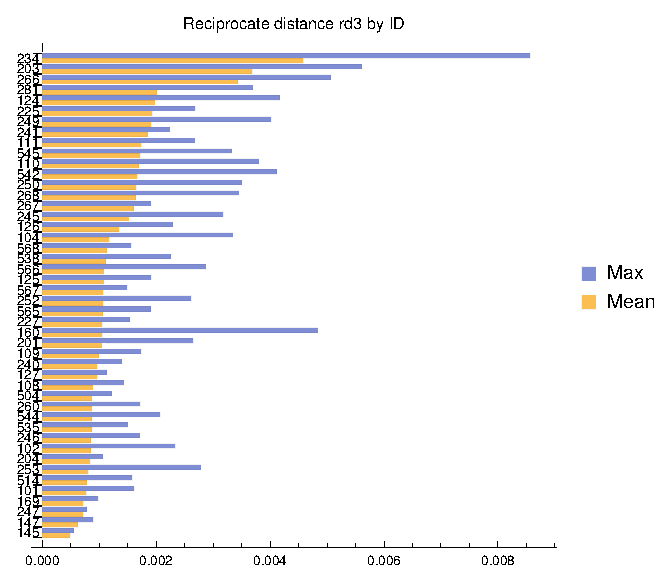
\includegraphics[clip,width=0.45\textwidth]{plots/HERA2_HERA2NoJet/rd3/CT14HERA2NNLOall_AbsSens_newSens_formula_cutbrokenpoints/residual_all_norm_Reciprocate_distance_ID_max_mean}
\ \ \
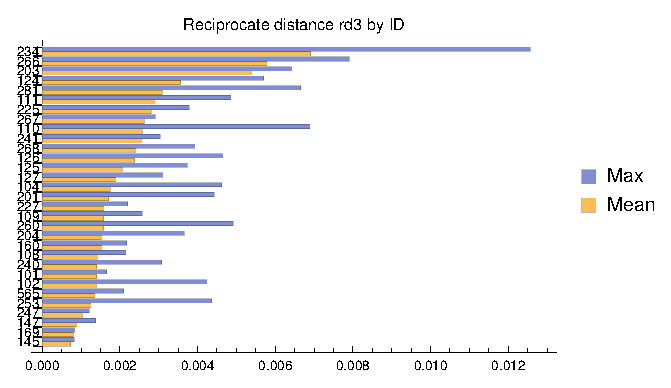
\includegraphics[clip,width=0.45\textwidth]{plots/HERA2_HERA2NoJet/rd3/HERA2_no_jet/residual_all_norm_Reciprocate_distance_ID_max_mean} 

\caption{reciprocate distance among residual/norm of points in data sets. left-up:
HERA2 reciprocate distance. right-up: HERA2NoJet reciprocate distance.
left-down: mean and max of reciprocate distances by experiments, HERA2.
right-down: mean and max of reciprocate distances by experiments,
HERA2.}
\label{fig:HERA2_HERA2NoJet_rd3}
\end{figure*}

\begin{figure*}
\includegraphics[clip,width=0.45\textwidth]{plots/HERA2_HERA2NoJet/tensorprojector/pca}
\ \ \
\includegraphics[clip,width=0.45\textwidth]{plots/HERA2_HERA2NoJet/tensorprojector/tsne}

\caption{Distributions of displaced residuals $\vec{\delta_{i}}$ from the
CTEQ-TEA analysis obtained by dimensionality reduction methods. Left:
a 3-dimensional projection of a 10-dimensional manifold constructed
by principal component analysis (PCA). Right: a distribution from
the 3-dimensional t-SNE clustering method. Blue, orange, and red colors
indicate data points from DIS, vector boson production, and jet/$t\bar{t}$
production processes.}
\label{fig:PCA_t-SNE} 
\end{figure*}

\section{Other researches }

\subsection{Quantifying the sensitivity to PDFs in a x-range }

\subsection{construct theoretical predictions are the linear combination of different
flavour PDFs }

\section{Conclusions \label{sec:Conclusions}}

......

\subsection*{Acknowledgements}

......\bibliographystyle{apsrev}
\bibliography{PDFsense_material}
 

\appendix

\section{Approximate kinematical variables\label{sec:supp}}

......

\section{Tabulated results \label{sec:Tables}}

......

\onecolumngrid
\begin{table}
\begin{tabular}{|l|lr|c|}
\hline 
\textbf{ID\#}  & \textbf{Experimental data set}  &  & $N_{pts}$ \tabularnewline
\hline 
101  & BCDMS $F_{2}^{p}$  & \cite{Benvenuti:1989rh}  & 337 \tabularnewline
\hline 
102  & BCDMS $F_{2}^{d}$  & \cite{Benvenuti:1989fm}  & 250 \tabularnewline
\hline 
104  & NMC $F_{2}^{d}/F_{2}^{p}$  & \cite{Arneodo:1996qe}  & 123 \tabularnewline
\hline 
108  & CDHSW $F_{2}^{p}$  & \cite{Berge:1989hr}  & 85 \tabularnewline
\hline 
109  & CDHSW $F_{3}^{p}$  & \cite{Berge:1989hr}  & 96 \tabularnewline
\hline 
110  & CCFR $F_{2}^{p}$  & \cite{Yang:2000ju}  & 69 \tabularnewline
\hline 
111  & CCFR $xF_{3}^{p}$  & \cite{Seligman:1997mc}  & 86 \tabularnewline
\hline 
124  & NuTeV $\nu\mu\mu$ SIDIS  & \cite{Mason:2006qa}  & 38 \tabularnewline
\hline 
125  & NuTeV $\bar{\nu}\mu\mu$ SIDIS  & \cite{Mason:2006qa}  & 33 \tabularnewline
\hline 
126  & CCFR $\nu\mu\mu$ SIDIS  & \cite{Goncharov:2001qe}  & 40 \tabularnewline
\hline 
127  & CCFR $\bar{\nu}\mu\mu$ SIDIS  & \cite{Goncharov:2001qe}  & 38 \tabularnewline
\hline 
145  & H1 $\sigma_{r}^{b}$ ($57.4\mbox{ pb}^{-1}$)  & \cite{Aktas:2004az}\cite{Aktas:2005iw}  & 10 \tabularnewline
\hline 
147  & Combined HERA charm production ($1504\mbox{ pb}^{-1}$)  & \cite{Abramowicz:1900rp}  & 47 \tabularnewline
\hline 
160  & HERA1+2 Combined NC and CC DIS ($1\mbox{ fb}^{-1}$)  & \cite{Abramowicz:2015mha}  & 1120 \tabularnewline
\hline 
169  & H1 $F_{L}$ ($121.6\mbox{ pb}^{-1}$)  & \cite{Collaboration:2010ry}  & 9 \tabularnewline
\hline 
\end{tabular}\caption{Experimental data sets considered as part of CT14HERA2 and included
in this analysis: deep-inelastic scattering. \label{tab:EXP_1} }
\end{table}

\begin{table}
\begin{tabular}{|l|lr|c|}
\hline 
\textbf{ID\#}  & \textbf{Experimental data set}  &  & $N_{pts}$ \tabularnewline
\hline 
\hline 
201  & E605 DY  & \cite{Moreno:1990sf}  & 119 \tabularnewline
\hline 
203  & E866 DY, $\sigma_{pd}/(2\sigma_{pp})$  & \cite{Towell:2001nh}  & 15 \tabularnewline
\hline 
204  & E866 DY, $Q^{3}d^{2}\sigma_{pp}/(dQdx_{F})$  & \cite{Webb:2003ps}  & 184 \tabularnewline
\hline 
225  & CDF Run-1 $A_{e}(\eta^{e})$ ($110\mbox{ pb}^{-1}$)  & \cite{Abe:1996us}  & 11 \tabularnewline
\hline 
227  & CDF Run-2 $A_{e}(\eta^{e})$ ($170\mbox{ pb}^{-1}$)  & \cite{Acosta:2005ud}  & 11 \tabularnewline
\hline 
234  & D$\emptyset$~ Run-2 $A_{\mu}(\eta^{\mu})$ ($0.3\mbox{ fb}^{-1}$)  & \cite{Abazov:2007pm}  & 9 \tabularnewline
\hline 
240  & LHCb 7 TeV $W/Z$ muon forward-$\eta$ Xsec ($35\mbox{ pb}^{-1}$)  & \cite{Aaij:2012vn}  & 14 \tabularnewline
\hline 
241  & LHCb 7 TeV $W$ $A_{\mu}(\eta^{\mu})$ ($35\mbox{ pb}^{-1}$)  & \cite{Aaij:2012vn}  & 5 \tabularnewline
\hline 
260  & D$\emptyset$~ Run-2 $Z$ $d\sigma/dy_{Z}$ ($0.4\mbox{ fb}^{-1}$)  & \cite{Abazov:2006gs}  & 28 \tabularnewline
\hline 
261  & CDF Run-2 $Z$ $d\sigma/dy_{Z}$ ($2.1\mbox{ fb}^{-1}$)  & \cite{Aaltonen:2010zza}  & 29 \tabularnewline
\hline 
266  & CMS 7 TeV $A_{\mu}(\eta)$ ($4.7\mbox{ fb}^{-1}$)  & \cite{Chatrchyan:2013mza}  & 11 \tabularnewline
\hline 
267  & CMS 7 TeV $A_{e}(\eta)$ ($840\mbox{ pb}^{-1}$)  & \cite{Chatrchyan:2012xt}  & 11 \tabularnewline
\hline 
268  & ATLAS 7 TeV $W/Z$ Xsec, $A_{\mu}(\eta)$ ($35\mbox{ pb}^{-1}$)  & \cite{Aad:2011dm}  & 41 \tabularnewline
\hline 
281  & D$\emptyset$~ Run-2 $A_{e}(\eta)$ ($9.7\mbox{ fb}^{-1}$)  & \cite{D0:2014kma}  & 13 \tabularnewline
\hline 
504  & CDF Run-2 incl. jet ($d\sigma/dp_{T}^{j}dy_{j}$) ($1.13\mbox{ fb}^{-1}$)  & \cite{Aaltonen:2008eq}  & 72 \tabularnewline
\hline 
514  & D$\emptyset$~ Run-2 incl. jet ($d\sigma/dp_{T}^{j}dy_{j}$) (???)
($0.7\mbox{ fb}^{-1}$)  & \cite{Abazov:2008ae}  & 110 \tabularnewline
\hline 
535  & ATLAS 7 TeV incl. jet ($d\sigma/dp_{T}^{j}dy_{j}$) ($35\mbox{ pb}^{-1}$)  & \cite{Aad:2011fc}  & 90 \tabularnewline
\hline 
538  & CMS 7 TeV incl. jet ($d\sigma/dp_{T}^{j}dy_{j}$) ($5\mbox{ fb}^{-1}$)  & \cite{Chatrchyan:2012bja}  & 133 \tabularnewline
\hline 
\end{tabular}\caption{Same as Table~\ref{tab:EXP_1}, showing experimental data sets for
production of vector bosons, single-inclusive jets, and $t\bar{t}$
pairs. \label{tab:EXP_2} }
\end{table}

\begin{table}
\begin{tabular}{|l|lr|c|}
\hline 
\textbf{ID\#}  & \textbf{Experimental data set}  &  & $N_{pts}$ \tabularnewline
\hline 
\hline 
245  & LHCb 7 TeV Z/W muon forward-$\eta$ Xsec ($1.0\mbox{ fb}^{-1}$)  & \cite{Aaij:2015gna}  & 33 \tabularnewline
\hline 
246  & LHCb 8 TeV Z electron forward-$\eta$ $d\sigma/dy_{Z}$ ($2.0\mbox{ fb}^{-1}$)  & \cite{Aaij:2015vua}  & 17 \tabularnewline
\hline 
247  & ATLAS 7 TeV $d\sigma/dp_{T}^{Z}$ ($4.7\mbox{ fb}^{-1}$)  & \cite{Aad:2014xaa}  & 8 \tabularnewline
\hline 
249  & CMS 8 TeV W muon, Xsec, $A_{\mu}(\eta^{\mu})$ ($18.8\mbox{ fb}^{-1}$)  & \cite{Khachatryan:2016pev}  & 33 \tabularnewline
\hline 
250  & LHCb 8 TeV W/Z muon, Xsec, $A_{\mu}(\eta^{\mu})$ ($2.0\mbox{ fb}^{-1}$)  & \cite{Aaij:2015zlq}  & 42 \tabularnewline
\hline 
252  & ATLAS 8 TeV Z ($d^{2}\sigma/d|y|_{ll}dm_{ll}$) ($20.3\mbox{ fb}^{-1}$)  & \cite{Aad:2016zzw}  & 48 \tabularnewline
\hline 
253  & ATLAS 8 TeV ($d^{2}\sigma/dp_{T}^{Z}dm_{ll}$) ($20.3\mbox{ fb}^{-1}$)  & \cite{Aad:2015auj}  & 45 \tabularnewline
\hline 
542  & CMS 7 TeV incl. jet, R=0.7, ($d\sigma/dp_{T}^{j}dy_{j}$) ($5\mbox{ fb}^{-1}$)  & \cite{Chatrchyan:2014gia}  & 158 \tabularnewline
\hline 
544  & ATLAS 7TeV incl. jet, R=0.6, ($d\sigma/dp_{T}^{j}dy_{j}$) ($4.5\mbox{ fb}^{-1}$)  & \cite{Aad:2014vwa}  & 140 \tabularnewline
\hline 
545  & CMS 8TeV incl. jet, R=0.7, ($d\sigma/dp_{T}^{j}dy_{j}$) ($19.7\mbox{ fb}^{-1}$)  & \cite{Khachatryan:2016mlc}  & 185 \tabularnewline
\hline 
565  & ATLAS 8 TeV $t\overline{t}\:d\sigma/dp_{T}^{t}$ ($20.3\mbox{ fb}^{-1}$)  & \cite{Aad:2015mbv}  & 8 \tabularnewline
\hline 
566  & ATLAS 8 TeV $t\overline{t}\:d\sigma/dy_{<t/\overline{t}>}$ ($20.3\mbox{ fb}^{-1}$)  & \cite{Aad:2015mbv}  & 5 \tabularnewline
\hline 
567  & ATLAS 8 TeV $t\overline{t}\:d\sigma/dm_{t\overline{t}}$ ($20.3\mbox{ fb}^{-1}$)  & \cite{Aad:2015mbv}  & 7 \tabularnewline
\hline 
568  & ATLAS 8 TeV $t\overline{t}\:d\sigma/dy_{t\overline{t}}$ ($20.3\mbox{ fb}^{-1}$)  & \cite{Aad:2015mbv}  & 5 \tabularnewline
\hline 
\end{tabular}\caption{Same as Table~\ref{tab:EXP_1}, showing experimental data sets for
production of vector bosons, single-inclusive jets, and $t\bar{t}$
pairs that were not incorporated in the CT14HERA2 fit but included
in the augmented CTEQ-TEA set that informs our sensitivity figures
in the present analysis. \label{tab:EXP_3} }
\end{table}

% . . . . . TAB_4

%-   -   -    -    -    -    -    -    -    -    -    -   -   -    -    -    -    -    -    -    -    -    -    -   -   -    -    -    -    -    -    -    -    -

% . . . . . TAB_5

% . . . . . TAB_5
-
\end{document}
